%Januar 2021 - März 2021


\documentclass[12pt]{article}

\usepackage{multicol}
\usepackage{geometry}
\usepackage{blindtext}
\usepackage{setspace}
\usepackage{hyperref}
\usepackage[headsepline=0.8pt, footsepline =0.8pt]{scrlayer-scrpage}
\usepackage{listings}
\usepackage{subcaption}
\usepackage{tabularx}
\usepackage{xurl} %Formats \url{}-entrys better
\usepackage{color, colortbl}
%\usepackage{pdfpages}
\usepackage{amssymb}
\usepackage{caption}
\usepackage{subcaption}



\geometry{a4paper, top=25mm, left=35mm, right=25mm, bottom=25mm, headsep=13mm, footskip=12mm, head=14.5pt}

%encoding
%--------------------------------------
\usepackage[utf8]{inputenc}
\usepackage[T1]{fontenc}
%--------------------------------------

%German-specific commands
%--------------------------------------
\usepackage[ngerman]{babel}
%--------------------------------------

%Hyphenation rules
%--------------------------------------
\usepackage{hyphenat}
%--------------------------------------


\usepackage{graphicx}
\graphicspath{ bilder/}

\newcommand{\Autor}{Andreas Schmider}

\newcommand{\Bearbeitungszeitraum}{2 Semester}
\newcommand{\Kurs}{TINF19B3}
\newcommand{\Betreuer}{Prof. Dr.-Ing. Kai Becher}

\newcommand{\DHBWLogoDeckblatt}{
\includegraphics[width=4.5cm]{Logos/dhbw-logo}}
\newcommand{\KernPackages}{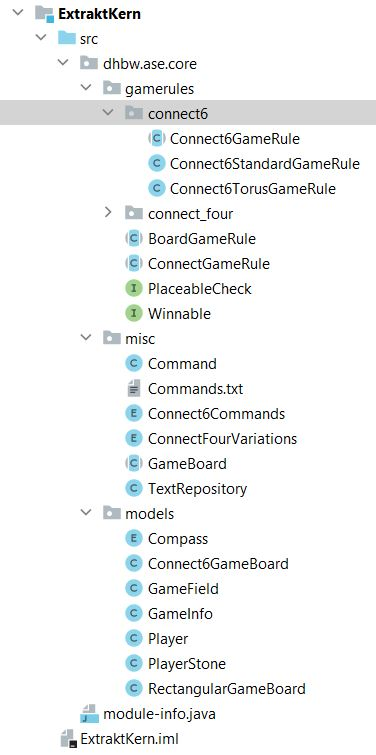
\includegraphics[height=12cm]{Bilder/KernModul_Packages}}
\newcommand{\PluginPackages}{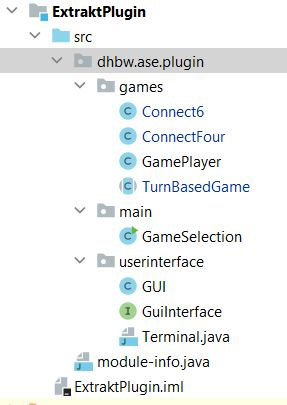
\includegraphics[height=7cm]{Bilder/PluginModul_Packages}}

\newcommand{\Titel}{Kleine Spielesammlung von 4-Gewinnt Versionen}
\newcommand{\ArtArbeit}{Studienarbeit}
\newcommand{\Abschluss}{Bachelor of Science}
\newcommand{\Studiengang}{Studiengang Informationstechnik}

\newcommand{\Ort}{Karlsruhe}

%\newcommand{\Abgabedatum}{16.02.2021}


\begin{document}
\onehalfspacing
\pagenumbering{Roman}
	\begin{titlepage}
		{\DHBWLogoDeckblatt}\\[2cm]
		\begin{center}
			\vspace*{-2cm}
			{\Huge \Titel}\\[2cm]
			{\Large \Abschluss}\\[0.5cm]
			{\large \Studiengang}\\[0.5cm]
			{\large an der}\\[0.5cm]
			{\large Dualen Hochschule Baden-Württemberg Karlsruhe}\\[0.5cm]
			{\large von}\\[0.5cm]
			{\large\bfseries \Autor}\\[1cm]
			{\large Abgabedatum 30. April 2022}
			\vfill
		\end{center}
		\begin{tabular}{l@{\hspace{1cm}}l}
			Bearbeitungszeitraum & \Bearbeitungszeitraum \\
			Kurs & \Kurs \\
		\end{tabular}
	\end{titlepage}

\newpage

\thispagestyle{empty}
\begin{center}
\Large\bfseries Erklärung
\end{center}
\medskip
\noindent
Wir versichern hiermit, dass wir unsere \ArtArbeit \ mit
dem Thema: 
\begin{center}
	 \Titel \ 
\end{center}
selbstständig verfasst und keine anderen als die angegebenen Quellen und
Hilfsmittel benutzt haben. Wir versichern zudem, dass die eingereichte elektronische Fassung mit der
gedruckten Fassung übereinstimmt.

\vspace{3cm}
\noindent
\underline{\Ort, 30. April 2022 \hspace{9cm}}\\
%\hfill\underline{\hspace{6cm}}\\
Ort, Datum\hfill Unterschrift\hspace{4cm}

\newpage

\thispagestyle{empty}
\tableofcontents

\newpage

%\thispagestyle{empty}
\thispagestyle{plain}
\cleardoublepage
\addcontentsline{toc}{section}{\listfigurename}
\listoffigures

\addcontentsline{toc}{section}{\listtablename}
\listoftables

\newpage


\thispagestyle{plain}
\pagenumbering{arabic}

\section{Beschreibung der Software}

\textbf{Beschreibung der Funktionalität}
\\
\noindent Aus einem alten Projekt existiert schon ein Connect6 Spiel, das in der Konsole gespielt wird. Dabei
gibt es einige Einstellungen die während des Programms noch gesetzt werden können. Somit kann
es von zwei bis vier Spielern gespielt oder die Spielfeldgröße auf 18x18 oder 20x20
festgelegt werden. Eine der größeren Auswirkung hat die Auswahl der Spielregeln.
Connect6 ist ähnlich wie Vier gewinnt und Ziel ist es mehrere Steine in eine Reihe zu legen.
Connect6 wird dabei aber auf einem Brett gespielt, das eben auf dem Boden liegt. So fallen die
Steine nicht bis in die letzte Zeile sondern bleiben an ihrem Platz. Ebenso werden pro Zug zwei
Steine pro Spieler gesetzt.
Bei der Standart-Spielregel zählen die Steine nur bis zum Spielfeldrand. Es gibt aber auch die
Torus-Version, bei dem die Steinreihen über den Rand hinaus gezählt werden. So beginnt das
Spielfeld erneut von oben, wenn man aus der untersten Zeile eins nach unten gehen würde.
\\

Zusätzlich dazu soll jetzt auch noch Vier Gewinnt mit unterschiedlichen Variationen/Regeln implementiert werden. Bei einer Variation soll es möglich sein, die Spielsteine nur von oben herunterfallen zu lassen. Bei einer anderen z.B. Drop Four ist es aber auch möglich den untersten Stein einer Spalte zu entfernen.
Bei dieser Spielesammlung soll es möglich sein mit wenig Aufwand neue Spielregeln/Variationen 
oder sogar ganz neue Spiele (die einen ähnlichen Aufbau haben) zu implementieren.
\\

Bei der Entwicklung dieser Software wurde zwar darauf geachtet einen möglichst strukturierten und einfachen Code zu erstellen,
es wurde sich aber nicht direkt an die in dieser Vorlesung besprochenen Themen gehalten. Es wurde zwar versucht die DRY-Regel anzuwenden, 
da diese mir schon selber in den Sinn gekommen ist, aber wie ich später festgestellt habe wurde diese nicht überall umgesetzt. Ebenso habe ich öfters kleinere Code Reviews vorgenommen und refactored, da mir immer wieder beim erneuten Anschauen aufgefallen ist, wie unverständlich der Code ist. Da der Code ursprünglich von einer Programmieraufgabe am KIT stammt, mussten auch Kommentare verwendet werden. Nachdem ich diesen Code aber nach über 3 Jahren wieder angeschaut habe ist mir klar geworden, dass trotz vieler Kommentare der Code sehr schwierig zu lesen ist.
\\ 

\noindent  \textbf{Beschreibung des Kundennutzens}
Der Kunde erhält Spaß und Unterhaltung.
\\

\noindent \textbf{Verwendete Technologien}
- Java
- JUnit 5
- IntelliJ
\\

\noindent \textbf{Link zum Repository}
\url{https://github.com/a-schmider/ASE_Substrat}

\newpage
\section{Unit tests}

\newpage
\section{Programming Principles}

\newpage
\section{Clean Architecture}
Dieses Programm wurde in zwei Schichten aufgeteilt. Dem Kern-Modul, in dem die ganzen Strukturen liegen, und dem Plugin-Modul, in dem momentan die Ausgabe/GUI realisiert wird. Um sicherzustellen, dass die Klassen im Kern die Plugins nicht kennen wurden Java Module verwendet und es wurde nur dem Plugin Modul gestattet die Klassen des Kerns zu verwenden und nicht andersherum. Dies ist wichtig, damit die Plugins ausgetauscht werden können ohne den Domain Code anpassen zu müssen.
\\

\begin{figure}[htpb!]
\centering
\begin{subfigure}{.5\textwidth}
  \centering
  {\KernPackages}\\[2cm]
  %\caption{A subfigure}
  \label{fig:sub1}
\end{subfigure}%
\begin{subfigure}{.5\textwidth}
  \centering
  {\PluginPackages}\\[2cm]
  %\caption{A subfigure}
  \label{fig:sub2}
\end{subfigure}
\caption{Kern- und Plugin-Module}
\label{fig:test}
\end{figure}





\newpage
\section{Entwurfsmuster}

\newpage
\section{Refactoring}


\end{document}